\ExerciseChapter{重复测量资料的方差分析}

\label{chapter:4}

\section{往年题}

\subsection{单项选择题}

\par\addvspace{6pt}\noindent\begin{minipage}{\linewidth}

\Question{E17-M8}{不等间隔的重复测量}

重复测量资料,如果重复测量的时间间隔不等,则适宜的综合指标是


\begin{choices}

\item 有峰型资料用均数

\item 生长型资料用极值

\item 均可使用最后的时点测量值

\item 有峰型资料用曲线下面积

\item 生长型资料用均数

\end{choices}

\end{minipage}\par\vspace{4pt}

\par\addvspace{6pt}\noindent\begin{minipage}{\linewidth}

\Question{E17-M10}{把重复观测当独立样本}

将n个患者的k次不同观察作因变量,样本含量为nk,用方差分析或GLM模型分析,可能出现的统计问题主要是


\begin{choices}

\item 降低了检验效能

\item 不易控制混杂因子

\item 信息利用率降低

\item 增加了I型错误概率

\item 无法分析时间趋势

\end{choices}

\end{minipage}\par\vspace{4pt}

\par\addvspace{6pt}\noindent\begin{minipage}{\linewidth}

\Question{E17-M11}{综合指标法与重复测量模型}

重复测量资料的综合指标法与GLM法,正确的理解是


\begin{choices}

\item 综合指标效率高

\item GLM法效率高

\item 总是GLM法较好

\item 总是综合指标法较好

\item 二者均不好,宜使用多重回归法分析

\end{choices}

\end{minipage}\par\vspace{4pt}

\par\addvspace{6pt}\noindent\begin{minipage}{\linewidth}

\Question{E17-M16}{给药途径与浓度轨迹}

某激素类药的不同给药途径的临床药代学及药效学研究,对两组病人采用不同给药途径,分别于给药即刻,1h,4h,12h,24h,测量其靶器官浓度并记录相应的疗效指标,数据分析宜使用


\begin{choices}

\item 分组散点图。

\item 边际均数图。

\item 偏回归图。

\item QQ图。

\item 残差分布图。

\end{choices}

\end{minipage}\par\vspace{4pt}

\par\addvspace{6pt}\noindent\begin{minipage}{\linewidth}

\Question{E17-M20}{血药浓度与时间因素}

药物动力学研究,考察给药后多个时点的血药浓度,分析其中某影响因素时宜使用


\begin{choices}

\item 分组散点图。

\item 边际均数图。

\item 偏回归图。

\item QQ图。

\item 残差分布图。

\end{choices}

\end{minipage}\par\vspace{4pt}

\Needspace{7\baselineskip}\subsubsection*{共用资料：早产儿配方奶与肠道菌群}

原题引用 Addition of gangliosides to an adapted milk formula modifies levels of fecal Escherichia coli in preterm newborn infants（Rueda等，1998，PMID 9672517）。已核对题名和公开摘要，但原题所需Fig.2与Table 2完整数值未提供；摘要不能替代这些图表。


\par\addvspace{6pt}\noindent\begin{minipage}{\linewidth}

\Question{E17-L6}{由原图重算卡方P值}

Fig.2, Days 3, Chi-square test,其P值是


\begin{choices}

\item 0.068

\item 0.088

\item 0.091

\item 0.096

\item 0.176

\end{choices}

\end{minipage}\par\vspace{4pt}

\par\addvspace{6pt}\noindent\begin{minipage}{\linewidth}

\Question{E17-L7}{哪种菌有组与时间交互}

Table 2, 如果使用GLM of repeated measurements,则group*day最有可能有统计学意义的菌类是


\begin{choices}

\item Coliforms

\item E.coli

\item Total aerobes

\item Bifidobacteria

\item E.coli and Bifidobacteria

\end{choices}

\end{minipage}\par\vspace{4pt}

\par\addvspace{6pt}\noindent\begin{minipage}{\linewidth}

\Question{E17-L8}{用AUC比较菌群过程}

Table 2,适宜使用曲线下面积进行综合指标分析,且可能得到有统计学意义结果的菌类是


\begin{choices}

\item Coliforms

\item E.coli

\item Total aerobes

\item Bifidobacteria

\item Enterobacteria

\end{choices}

\end{minipage}\par\vspace{4pt}

\par\addvspace{6pt}\noindent\begin{minipage}{\linewidth}

\Question{E17-L9}{重复测量分析的主要问题}

本文有关统计分析存在最主要的问题是


\begin{choices}

\item 统计效率不高结果解释困难

\item 用Mean±SEM展示数据

\item 样本量小

\item 图1令人费解

\item 同时使用Kruskal-walis test and Friedman test

\end{choices}

\end{minipage}\par\vspace{4pt}

\par\addvspace{6pt}\noindent\begin{minipage}{\linewidth}

\Question{E21-16}{错误独立化后的方差分解}

将n个患者的k次不同观察作因变量视为nk个样本做普通方差分析,则在分析组间效应时,与重复测量方差分析不同之处有 I、误差平方和不同 II、误差自由度不同 III、组间或个体间均方不同(错,相同)


\begin{choices}

\item I

\item I\&II

\item I\&III

\item II\&III

\item I\&II\&III

\end{choices}

\end{minipage}\par\vspace{4pt}

\par\addvspace{6pt}\noindent\begin{minipage}{\linewidth}

\Question{E21-17}{单变量重复测量的条件}

关于重复测量资料做一元方差分析需要满足的条件,正确的说法是


\begin{choices}

\item 需满足Mauchly's Sphericity条件,否则需要校正

\item 需满足Compound Symmetry条件,否则需要校正

\item 需满足Huyhn-Feldt条件,否则需要校正

\item 需满足Greenhouse-Geisser条件,否则需要校正

\item 需满足Equal Variance条件,否则需要校正

\end{choices}

\end{minipage}\par\vspace{4pt}

\par\addvspace{6pt}\noindent\begin{minipage}{\linewidth}

\Question{E21-18}{标准化Helmert对比}

下列哪些是标准化Helmert对比矩阵？ \[\mathrm{I}:\begin{pmatrix}1&-0.5&-0.5\\0&0.5&-0.5\end{pmatrix},\] \[\mathrm{II}:\begin{pmatrix}2/\sqrt6&-1/\sqrt6&-1/\sqrt6\\0&1/\sqrt2&-1/\sqrt2\end{pmatrix},\qquad
\mathrm{III}:\begin{pmatrix}2&-1&-1\\0&1&-1\end{pmatrix}.\]


\begin{choices}

\item 仅I。

\item 仅II。

\item 仅III。

\item I与III。

\item I、II与III。

\end{choices}

\end{minipage}\par\vspace{4pt}

\par\addvspace{6pt}\noindent\begin{minipage}{\linewidth}

\Question{E21-20}{重复测量平方和的层次}

重复测量资料的平方和分解,正确的说法有 I、个体间的变异含处理或组间的主效应 II、个体内的变异含处理和时间的交互作用 III、个体间的误差包含个体内的误差


\begin{choices}

\item I

\item II

\item III

\item I\&II

\item I\&II\&III

\end{choices}

\end{minipage}\par\vspace{4pt}

\par\addvspace{6pt}\noindent\begin{minipage}{\linewidth}

\Question{E21-12}{GG校正改变什么}

重复测量单变量检验采用Greenhouse--Geisser校正时，通常：


\begin{choices}

\item 改变原始观察值。

\item 将F统计量乘以epsilon。

\item 用epsilon同时调整相关F检验的分子与分母自由度，F值本身不变。

\item 删除所有不显著时点。

\item 把同一个体的测量强行视为独立。

\end{choices}

\end{minipage}\par\vspace{4pt}

\par\addvspace{6pt}\noindent\begin{minipage}{\linewidth}

\Question{N19-19}{两个时点的球形性}

只有两个完整重复测量时点时，球形条件：


\begin{choices}

\item 自动成立，因为只有一个独立差值维度。

\item 必然不成立。

\item 必须通过四维正态检验。

\item 必须要求每个Y完全相同。

\item 只有样本量超过100才成立。

\end{choices}

\end{minipage}\par\vspace{4pt}

\par\addvspace{6pt}\noindent\begin{minipage}{\linewidth}

\Question{N19-20}{按指定检验水平作决定}

Mauchly检验P=.065，题目规定前提检验水平=.20，应：


\begin{choices}

\item 拒绝球形性，考虑校正或其他适合方法。

\item 因P\textgreater.05而直接判满足题目条件。

\item 把P四舍五入为0。

\item 删除所有不满足的受试者。

\item 增大每个观测值。

\end{choices}

\end{minipage}\par\vspace{4pt}

\Needspace{7\baselineskip}\subsubsection*{共用资料：运动员激素资料的重复观测设计}

随附《三种口服避孕药对女运动员部分甲状腺轴激素的影响》随机分21名受试者至A、B、C三组（8、8、5人），在服药前后不同月经周期阶段反复测量TSH、T4、rT3等指标。各组部分采样日程不同，文章给出多个组别×时点均值及标准差。以下仅练习统计设计与解释，不作为选药建议。


\par\addvspace{6pt}\noindent\begin{minipage}{\linewidth}

\Question{N19-27}{激素试验的独立单位}

对运动员激素重复测量研究，通常独立实验单位是：


\begin{choices}

\item 受试者。

\item 每次抽血得到的一条数值。

\item 每种激素的名称。

\item 每个P值。

\item 每个时间点均值。

\end{choices}

\end{minipage}\par\vspace{4pt}

\par\addvspace{6pt}\noindent\begin{minipage}{\linewidth}

\Question{N19-28}{从激素结果到应用结论}

仅观察到某些激素在服药前后有变化，最稳妥的统计解释是：


\begin{choices}

\item 限定在所测指标和比较条件，不直接推断运动表现改善或完整临床使用价值。

\item 足以证明所有运动员都应采用该方案。

\item 足以证明未测的代谢率必然改变相同幅度。

\item 未显著的激素变化就证明药物完全无效应。

\item 可以忽略多指标、多时点的比较问题。

\end{choices}

\end{minipage}\par\vspace{4pt}

\par\addvspace{6pt}\noindent\begin{minipage}{\linewidth}

\Question{N19-29}{不等间隔AUC的计算}

时间为0、0.5、1、2小时，梯形法AUC正确做法是：


\begin{choices}

\item 每段平均高度乘该段实际时间宽度后求和。

\item 把4个数直接相加。

\item 将3段都当成1小时。

\item 只取最大值。

\item 用每组均值的一个AUC当作多个受试者。

\end{choices}

\end{minipage}\par\vspace{4pt}

\par\addvspace{6pt}\noindent\begin{minipage}{\linewidth}

\Question{N19-30}{球形条件的矩阵表述}

令H为标准正交的时间对比矩阵，球形性通常要求：


\begin{choices}

\item \(H\Sigma H^T=\sigma^2I\)。

\item \(\Sigma\)的所有元素为0。

\item 所有时点的均值相同。

\item 不同组均值相同。

\item 每个人的观测轨迹相同。

\end{choices}

\end{minipage}\par\vspace{4pt}

\subsection{简答题}

\par\addvspace{6pt}\noindent\begin{minipage}{\linewidth}

\Question{REF15-1}{为何经常采用重复测量设计}

为什么具有重复测量的设计在医学研究领域中被使用的频率相当高？


\worklines{3}

\end{minipage}\par\vspace{4pt}

\par\addvspace{6pt}\noindent\begin{minipage}{\linewidth}

\Question{REF15-2}{重复测量资料的收集规范}

人们在收集具有重复测量设计的资料时常犯什么错误？避免此类错误的办法是什么？


\worklines{3}

\end{minipage}\par\vspace{4pt}

\par\addvspace{6pt}\noindent\begin{minipage}{\linewidth}

\Question{REF15-3}{重复测量资料的本质区别}

重复测量设计资料与非重复测量设计资料的本质区别是什么？


\worklines{3}

\end{minipage}\par\vspace{4pt}

\par\addvspace{6pt}\noindent\begin{minipage}{\linewidth}

\Question{REF15-4}{识别与分析重复测量}

如何准确识别重复测量设计？处理重复测量数据的基本思路是什么？


\worklines{3}

\end{minipage}\par\vspace{4pt}

\subsection{计算与分析题}

\Question{C20-4}{家兔血钾的重复测量与综合指标}

15只家兔分成3个处理组，各5只，测量处理前及处理后0.5、1、2小时的血钾。研究目标是不同处理后的变化是否不同。数据文件为个人还原版，已与附带文献的表1逐行核对一致，数值按原单位保留。

\begin{center}\small\setlength{\tabcolsep}{3.5pt}\renewcommand{\arraystretch}{1.18}\begin{tabular}{@{}lrrrrr@{}}
\toprule
组 & 兔号 & 处理前 & 0.5h & 1h & 2h \\
\midrule

1 & 1 & 154.5 & 129.8 & 122.7 & 171.7 \\
1 & 2 & 173 & 124 & 170.4 & 168.6 \\
1 & 3 & 186 & 131 & 137 & 138 \\
1 & 4 & 161 & 154 & 178 & 128 \\
1 & 5 & 187 & 158 & 162 & 152 \\
2 & 6 & 144.4 & 135.5 & 149.9 & 129.1 \\
2 & 7 & 147.1 & 134.2 & 138.3 & 146.1 \\
2 & 8 & 183.6 & 189.3 & 190.5 & 227.3 \\
2 & 9 & 181.7 & 160.3 & 163.3 & 163.3 \\
2 & 10 & 166.7 & 136.8 & 134.6 & 142.5 \\
3 & 11 & 173.3 & 231.4 & 293.7 & 401.4 \\
3 & 12 & 155.1 & 199.6 & 191.8 & 203.4 \\
3 & 13 & 177.9 & 153.6 & 158.7 & 240.3 \\
3 & 14 & 158.2 & 146.7 & 135.2 & 228.7 \\
3 & 15 & 180.4 & 170.8 & 226.2 & 267.7 \\
\bottomrule\end{tabular}\end{center}

\begin{enumerate}
\def\labelenumi{\arabic{enumi}.}
\tightlist
\item
  检验H-F条件，球形检验水平0.2。
\item
  做单变量重复测量方差分析，效应检验水平0.05，必要时校正。
\item
  绘制分组时点均数图，说明结果。
\item
  去掉第3组，用SMA比较第1、2组的血钾平均变化量。
\end{enumerate}


\worklines{3}

\par\addvspace{6pt}\noindent\begin{minipage}{\linewidth}

\Question{C21-4}{Attention Blink的重复测量分析}

对Attention Blink数据（删去乒乓球选手组、保留三个研究组及8个位置指标）作分析： 1. 检验H-F条件，检验水平0.2。 2. 做单变量重复测量方差分析，效应水平0.05；需要时给出``CG校正''结果（本书按GG校正理解）。 3. 绘制各组的时点/刺激位置均数图并解释。

配套还原数据保留80、14、17人的三组。原始2023附件把后两组合在同一标签中，不应直接把该两组标签当作原题三组。


\worklines{3}

\end{minipage}\par\vspace{4pt}



\clearpage\section{补充练习}

本节为配合正文新编的补充练习，按题型排列，题号接续本章往年题，解析见章末。

\subsection{单项选择题}

\par\addvspace{6pt}\noindent\begin{minipage}{\linewidth}

\Question{X26-4-1}{区组与条件重复的识别}

以下哪些资料属于同一实验单位的重复测量？

I. 在每个科室内，将不同患者随机分到三种处理，每位患者仅测量一次结局。

\begin{enumerate}
\def\labelenumi{\Roman{enumi}.}
\setcounter{enumi}{1}
\item
  同一受试者依次戴三种不同镜片，分别测量同一项电反应延迟。
\item
  同一患者分别在给药前及给药后四个时点测量收缩压。
\end{enumerate}


\begin{choices}

\item 仅I。

\item 仅II。

\item 仅III。

\item II与III。

\item I、II与III。

\end{choices}

\end{minipage}\par\vspace{4pt}

\par\addvspace{6pt}\noindent\begin{minipage}{\linewidth}

\Question{X26-4-2}{协方差结构的判别}

三个重复测量时点的理论协方差阵为 \[\Sigma=\begin{pmatrix}4&1&2\\1&6&3\\2&3&8\end{pmatrix}.\] 以下判断正确的是：

I. 该矩阵具有复合对称（CS）结构。

\begin{enumerate}
\def\labelenumi{\Roman{enumi}.}
\setcounter{enumi}{1}
\item
  三个两两差值 \(Y_1-Y_2\)、\(Y_1-Y_3\)、\(Y_2-Y_3\) 的方差均为8。
\item
  该矩阵满足正文所称H-F条件（广义球形性）。
\end{enumerate}


\begin{choices}

\item 仅I。

\item 仅II。

\item II与III。

\item I与III。

\item I、II与III。

\end{choices}

\end{minipage}\par\vspace{4pt}

\par\addvspace{6pt}\noindent\begin{minipage}{\linewidth}

\Question{X26-4-3}{由对比协方差计算GG系数}

一组受试者有4个重复测量时点。对样本协方差阵作标准正交时间对比变换，所得 \(3\times3\) 协方差阵的特征值为1、1、4。按正文公式，Greenhouse-Geisser系数 \(\hat\varepsilon\) 为：


\begin{choices}

\item \(1/3\)。

\item \(1/2\)。

\item \(3/4\)。

\item \(1\)。

\item \(2/3\)。

\end{choices}

\end{minipage}\par\vspace{4pt}

\subsection{简答题}

\par\addvspace{6pt}\noindent\begin{minipage}{\linewidth}

\Question{X26-4-4}{多组资料为什么用合并残差协方差}

三组受试者分别有 \(n_1,n_2,n_3\) 人，每人均有5个时点的完整测量。拟按正文方法检验共同协方差阵的H-F条件。某同学不区分组别，直接用全部原始观测的 \(5\times5\) 协方差阵作检验。

说明这一做法可能混入什么变异；写出正文合并协方差阵的计算思路、分母自由度及应接受球形检验的矩阵维度。


\worklines{3}

\end{minipage}\par\vspace{4pt}

\clearpage

\subsection{计算与分析题}

\Question{X26-4-5}{麻醉诱导的重复测量输出填空}

15名受试者随机等分为A、B、C三组，在5个时点测量收缩压（mmHg），采用正文原表：

\begin{center}\small\setlength{\tabcolsep}{5pt}\renewcommand{\arraystretch}{1.18}\begin{tabular}{@{}lllllll@{}}
\toprule
组别 & 编号 & T0 & T1 & T2 & T3 & T4 \\
\midrule

A & 1 & 120 & 108 & 112 & 120 & 117 \\
A & 2 & 118 & 109 & 115 & 126 & 123 \\
A & 3 & 119 & 112 & 119 & 124 & 118 \\
A & 4 & 121 & 112 & 119 & 126 & 120 \\
A & 5 & 127 & 121 & 127 & 133 & 126 \\
B & 6 & 121 & 120 & 118 & 131 & 137 \\
B & 7 & 122 & 121 & 119 & 129 & 133 \\
B & 8 & 128 & 129 & 126 & 135 & 142 \\
B & 9 & 117 & 115 & 111 & 123 & 131 \\
B & 10 & 118 & 114 & 116 & 123 & 133 \\
C & 11 & 131 & 119 & 118 & 135 & 129 \\
C & 12 & 129 & 128 & 121 & 148 & 132 \\
C & 13 & 123 & 123 & 120 & 143 & 136 \\
C & 14 & 123 & 121 & 116 & 145 & 126 \\
C & 15 & 125 & 124 & 118 & 142 & 130 \\
\bottomrule\end{tabular}\end{center}

给出软件输出摘要：在合并残差的时间对比空间中，Mauchly \(W=0.2930746\)、\(P=0.1776608\)，\(\hat\varepsilon_{GG}=0.6786930\)。前提检验水平定为0.20，效应检验水平为0.05。

\begin{enumerate}
\def\labelenumi{\arabic{enumi}.}
\tightlist
\item
  指出组间因素、组内因素及独立受试者数；按题设水平判断是否需要球形性校正。
\item
  用原始数据填出``组别、个体间误差、时间、组别×时间、个体内误差''五项的平方和与自由度，并计算三个效应的未校正F值。
\item
  填出时间和交互作用GG校正后的分子、分母自由度，说明组别检验是否作相同校正。
\item
  计算各组在5个时点的均数，结合效应检验解释组间过程。若把前提检验水平改为0.05，是否仍须按该检验结果作GG校正？
\end{enumerate}


\worklines{3}

\clearpage\section{习题解析}

\begin{keyidea}[核对方式]题号与前文一一对应。补写范围、原题歧义及数据还原方法列在相应答案中。\end{keyidea}

\Answer{E17-M8}{不等间隔的重复测量}

\textbf{答案：D。}

峰形过程可用梯形法按实际间隔计算AUC；直接平均各时点会隐含等权，不能表达真实时间累计暴露。生长型过程也可用斜率等指标，选择须对应研究问题。


\Answer{E17-M10}{把重复观测当独立样本}

\textbf{答案：D。}

同一受试者的多次测量相关，按nk个独立单位计算会错误估计标准误和自由度，常导致组间效应检验的I类错误膨胀。有效独立受试者数仍是n。


\Answer{E17-M11}{综合指标法与重复测量模型}

\textbf{答案：B（一般经验，不是必然结论）。}

正确的重复测量模型利用完整时间结构，通常比压缩成单一指标保留更多信息。但预先选定且切合目标的综合指标可更稳健、更易解释；没有对所有数据均更优的方法，C、D的``总是''不成立。


\Answer{E17-M16}{给药途径与浓度轨迹}

\textbf{答案：B。}

边际均数图可展示各组在多个实际时点的平均浓度轨迹，并辅助解释组×时间交互；本图并非完整的推断方法。


\Answer{E17-M20}{血药浓度与时间因素}

\textbf{答案：B。}

边际均数图显示给定因素各水平下的平均时间过程；还应以合适的重复测量模型处理个体内相关。


\Answer{E17-L6}{由原图重算卡方P值}

\textbf{答案：原图缺失，不能确认选项。}

应从Day 3的实际计数构造列联表，并明确Pearson卡方是否作连续性校正，或是否改用精确检验。公开摘要不含Fig.2计数，不能从其他日期的显著性反推本题P值。


\Answer{E17-L7}{哪种菌有组与时间交互}

\textbf{答案：原表缺失，不能确认选项。}

组×时间交互检验的是两组时间曲线形状是否不同；某一时点显著或同组随时间显著都不能替代交互检验。需完整个体数据或足够的均值、协方差与样本量。


\Answer{E17-L8}{用AUC比较菌群过程}

\textbf{答案：原表缺失，不能确认选项。}

应按个体在实际时点计算AUC，再比较两组。不能仅用组均值曲线计算一个面积后当作拥有多个独立重复的样本；原摘要提及E.coli关联，但不足以确认本题的唯一选项。


\Answer{E17-L9}{重复测量分析的主要问题}

\textbf{答案：A是通常的评议方向，需全文核验。}

将多时点分别作组间和组内检验可能难以整体评价交互且有多重性问题，合适的重复测量或混合模型通常更易对应目标。均值±SEM本身不必然错误，但要说明它表达均值精度；不能仅凭方法名认定两种非参数检验并用必错。


\Answer{E21-16}{错误独立化后的方差分解}

\textbf{答案：B。}

同一个平衡完整数据表，组间效应平方和的计算可相同，但普通nk样本模型与重复测量模型使用的误差平方和、误差自由度不同。组间效应应以个体间误差检验，不能用混合了个体内变异的误差项。


\Answer{E21-17}{单变量重复测量的条件}

\textbf{答案：C是课程的H-F条件命名。}

通常所需为球形性：对比空间的协方差矩阵与单位阵成比例。Mauchly是检验名称；复合对称更强，并非必要条件。GG/HF通常是违反球形性后的自由度校正名。A若只想表达``满足球形性''也有道理，故这道题主要考术语，不能把它们误作互不相关的5种条件。


\Answer{E21-18}{标准化Helmert对比}

\textbf{答案：B。}

标准化Helmert对比每行和为0，行间正交，且每行长度为1。矩阵I行长度不同，III未单位化；II满足 \(HH^T=I_2\) 且 \(H\mathbf1=0\)。


\Answer{E21-20}{重复测量平方和的层次}

\textbf{答案：D。}

个体间变异含组效应及个体间误差；个体内变异含时间、组×时间及个体内误差。两种误差属于不同层次，个体间误差不包含个体内误差。


\Answer{E21-12}{GG校正改变什么}

\textbf{答案：C。}

GG校正通过自由度影响尾概率，不改变已计算的平方和与F比值。


\textbf{补写说明。} 原第12题整题未记录，本题新编。


\Answer{N19-19}{两个时点的球形性}

\textbf{答案：A。}

一维对比协方差天然是标量，仍需考虑不同个体独立等其他条件。


\textbf{补写说明。} 2019回忆稿只给出30道选择的总数及大致范围，没有记录本题原文；本题是依课程内容与所附材料新编的补充练习，不冒作恢复的原试卷。


\Answer{N19-20}{按指定检验水平作决定}

\textbf{答案：A。}

必须按题设水平判断；拒绝球形性后可以使用GG/HF自由度校正或合适的相关结构模型。


\textbf{补写说明。} 2019回忆稿只给出30道选择的总数及大致范围，没有记录本题原文；本题是依课程内容与所附材料新编的补充练习，不冒作恢复的原试卷。


\Answer{N19-27}{激素试验的独立单位}

\textbf{答案：A。}

同一人的多时点及多个指标会相关，不能把所有数值都当独立受试者；随机分组发生在受试者层面。

\textbf{附文献批注校正。} 批注建议把``服药前后''和``药物种类''视为两个组间因素；同一受试者前后反复观测时，前后实际上是组内因素，药物种类才是组间因素。周期内阶段也是重复因素，还需核对各组测量时间是否可比。不能因把数据排成长表，就将同一人的前后值当作独立组。


\textbf{补写说明。} 2019回忆稿只给出30道选择的总数及大致范围，没有记录本题原文；本题是依课程内容与所附材料新编的补充练习，不冒作恢复的原试卷。


\Answer{N19-28}{从激素结果到应用结论}

\textbf{答案：A。}

应区分已测结果与未测结局，考虑对照、周期变化、重复相关、多重性及不确定性。这里不对临床用药作建议。


\textbf{补写说明。} 2019回忆稿只给出30道选择的总数及大致范围，没有记录本题原文；本题是依课程内容与所附材料新编的补充练习，不冒作恢复的原试卷。


\Answer{N19-29}{不等间隔AUC的计算}

\textbf{答案：A。}

各段宽度为0.5、0.5、1；组间比较应先在每个独立个体层面计算指标。


\textbf{补写说明。} 2019回忆稿只给出30道选择的总数及大致范围，没有记录本题原文；本题是依课程内容与所附材料新编的补充练习，不冒作恢复的原试卷。


\Answer{N19-30}{球形条件的矩阵表述}

\textbf{答案：A。}

它约束个体内对比的协方差，不约束均值或处理效应。对比空间内更换正交基不应改变是否球形的结论。


\textbf{补写说明。} 2019回忆稿只给出30道选择的总数及大致范围，没有记录本题原文；本题是依课程内容与所附材料新编的补充练习，不冒作恢复的原试卷。


\Answer{REF15-1}{为何经常采用重复测量设计}

医学研究常关注病程、治疗反应、药代过程和生长发育的动态变化。同一受试者在多个时点观测可描述轨迹、比较变化，并利用个体内相关减少某些个体差异的影响，在合适设计下提高效率。反复测量的便利并不等于增加了同等数量的独立受试者，推断必须保留个体层次。


\Answer{REF15-2}{重复测量资料的收集规范}

常见问题包括丢失个体与时点对应、只保存各组均值而不留个体原始值、未记录实际间隔、把未测记成0、测量方法随时间改变而未注明。应保存唯一受试者ID、组别、实际时间、结局与缺失原因，统一测量流程，并能从宽表或长表还原每个人的完整观测序列。仅有均值和标准差通常不能重建个体内协方差。


\Answer{REF15-3}{重复测量资料的本质区别}

重复测量来自同一实验单位的多次观测，因此具有共同个体来源及相应的协方差结构；它包含个体间和个体内两个层次。是否属于重复测量应由设计和个体身份判定，而不是依据相关检验是否显著。非重复资料也可能有其他聚集相关，不能反过来认为它总是独立。


\Answer{REF15-4}{识别与分析重复测量}

先追溯实验单位：同一人、动物或其他独立单位在不同时间/条件下是否反复提供观测。明确组间因素、组内因素、实际时点和目标比较，再绘制个体及组均值轨迹，检查缺失。

分析可以是预先定义的SMA、合适的单变量重复测量方差分析及球形性校正、多变量方法或混合模型。需要使用正确的个体间/个体内误差，不能把正交变换理解为能够自动消除任意相关或``修好''球形性；模型应与设计、协方差结构和研究问题相符。


\Answer{C20-4}{家兔血钾的重复测量与综合指标}

对正确的个体内对比空间作Mauchly检验，\(W=0.378422\)，R的P约0.06523；在 \textbf{0.2} 水平拒绝球形性（若用0.05则结论不同）。未校正检验如下：

\begin{center}\small\setlength{\tabcolsep}{3.5pt}\renewcommand{\arraystretch}{1.18}\begin{tabular}{@{}lrrrr@{}}
\toprule
效应 & F & df1 & df2 & P \\
\midrule

组别 & 4.77741 & 2 & 12 & 0.029773 \\
时点 & 5.66101 & 3 & 36 & 0.002776 \\
组×时点 & 5.83597 & 6 & 36 & 0.000251 \\
\bottomrule\end{tabular}\end{center}

GG系数为0.654690，HF系数为0.781622。GG校正不改F值，时点自由度改为约(1.9641, 23.5688)，P=.01013；交互自由度改为(3.9281, 23.5688)，P=.00215。组别检验使用个体间误差，不因这项球形性校正改变。R与其他软件的Mauchly近似P可略有差别。

\begin{center}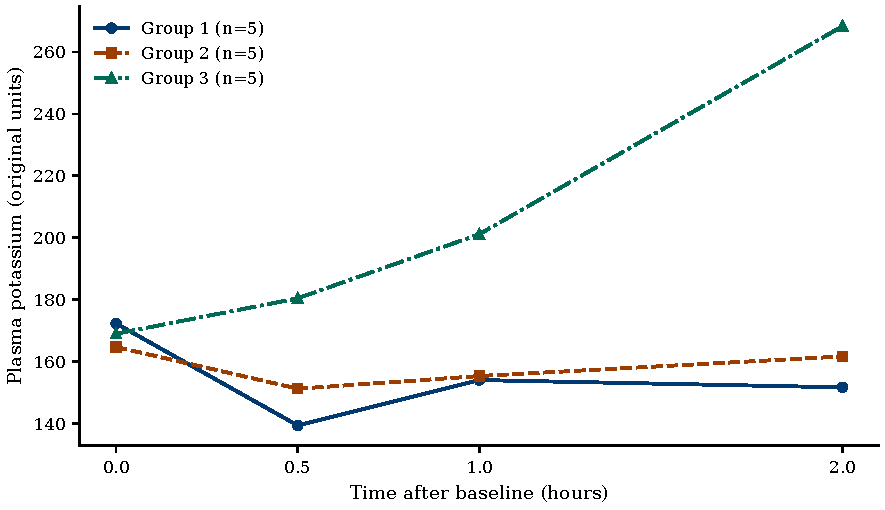
\includegraphics[width=.9\linewidth]{assets/rabbit_means.pdf}\end{center}

图为组均值，无置信区间；第3组后期明显上升，第1、2组相对平缓。交互有统计学证据，应优先描述不同时间过程，而非只给一个总体组差。

\textbf{SMA必须先定义指标。} 不等间隔下取基线校正曲线的时间平均变化 \[\Delta_i=\frac{1}{2}\int_0^2\{Y_i(t)-Y_i(0)\}\,dt,\] 积分以梯形法估计。第1、2组均值为−20.2500、−7.6475；Welch t=−1.3001，df\(\approx\) 7.999，P=.2298，差值95\% CI为(−34.956, 9.751)，证据不足。若按3个处理后时点直接平均再减基线，两组为−23.9533、−8.6333，P=.2025；若用个体线性斜率，P=.4758。原题``平均变化量''未唯一规定算法，应说明所采用的SMA定义，不能混淆变化量与变化率。


\Answer{C21-4}{Attention Blink的重复测量分析}

还原依据：正文的134人资料中删去原组2（23名乒乓球选手），剩余111行的8个观测值与2023附件逐值一致；保留原组1、3、4后重标为1、2、3，各均数与回忆稿完全相符。原附件未改写，还原CSV单独提供。

Mauchly \(W=0.074145\)，\(P\approx1.04\times10^{-42}\)，不满足球形性。GG系数0.514766，HF系数0.534728。以III型平方和为明确约定：

\begin{center}\small\setlength{\tabcolsep}{3.5pt}\renewcommand{\arraystretch}{1.18}\begin{tabular}{@{}lrrrrr@{}}
\toprule
效应 & F & 原df1 & 原df2 & 原P & GG校正P \\
\midrule

组别 & 1.57722 & 2 & 108 & 0.21127 & 不适用 \\
位置 & 42.38643 & 7 & 756 & \textless.001 & 2.84e-27 \\
组×位置 & 0.75126 & 14 & 756 & 0.72266 & 0.63241 \\
\bottomrule\end{tabular}\end{center}

位置校正自由度为约(3.6034, 389.1630)，交互为(7.2067, 389.1630)。原代码aov的顺序平方和与III型在不平衡组数下可检验不同加权主效应；本包同时保留aov输出，比较时不要混用。

\begin{center}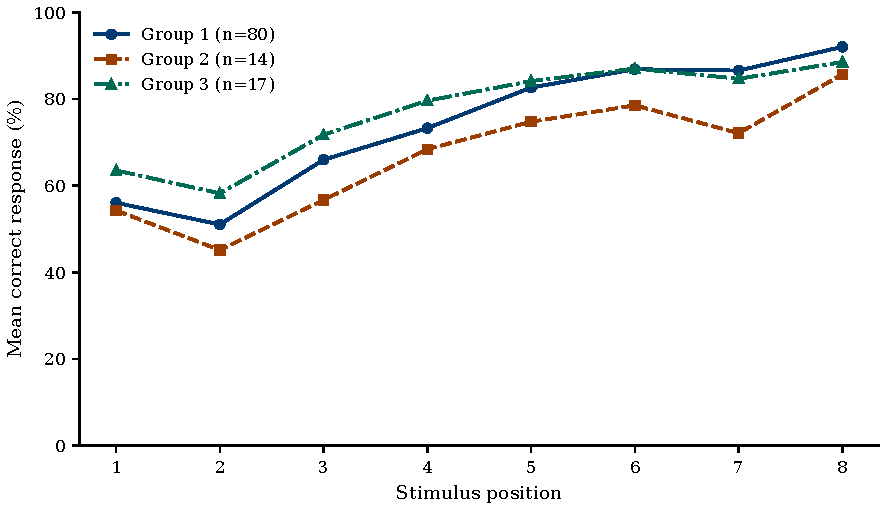
\includegraphics[width=.9\linewidth]{assets/attention_means.pdf}\end{center}

图只显示各组算术均值。p1---p8是刺激位置，原题没有给出足够信息换算成绝对时间。存在明显的位置变化，但组别及组×位置没有统计学证据；``不显著''不等于证明各组等效。

\clearpage\subsection*{补充练习解析}

以下为补充练习的解析。这些题目为配合正文新编，并非往年试题；题中设定的数值仅供练习。

\Answer{X26-4-1}{区组与条件重复的识别}

\textbf{答案：D。}

II是在同一人不同条件下重复测量，III是在同一人不同时点重复测量。I是区组内不同患者接受处理，每个人只提供一次结局；``有三种处理''不等于``同一人测三次''。是否重复须追溯实验单位，而不是只看资料按几列排列。




\Answer{X26-4-2}{协方差结构的判别}

\textbf{答案：C。}

三个差值方差分别为 \(4+6-2\times1=8\)、\(4+8-2\times2=8\)、\(6+8-2\times3=8\)，故II成立，也满足球形性对比条件。其对角元素不等、非对角元素也不等，不是CS结构。

若C的行是单位正交对比，\(C\mathbf1=0\)、\(CC^T=I_2\)，可验证 \(C\Sigma C^T=4I_2\)，所以III成立。本题区分原矩阵 \(\sigma^2I\)、CS与对比空间的广义球形性，不能把CS当作后者的必要条件。




\Answer{X26-4-3}{由对比协方差计算GG系数}

\textbf{答案：E。}

共有 \(4-1=3\) 个对比维度，故 \[\hat\varepsilon=\frac{(1+1+4)^2}{(4-1)(1^2+1^2+4^2)}=\frac{36}{54}=\frac23.\] 不能把分母中的``时点数减1''误写成4。应使用对比协方差阵的特征值；算出校正系数本身也不等于已完成球形性检验。




\Answer{X26-4-4}{多组资料为什么用合并残差协方差}

全部原始观测的协方差阵可能混入不同组均值轨迹之间的变异。正文的做法是先在各组、各时点减去相应组均数，计算组内协方差，再按组内自由度合并。若各组的理论协方差阵可视为共同的 \(\Sigma\)，则 \[S_{\mathrm{pool}}=\frac{\sum_{g=1}^{3}(n_g-1)S_g}{N-3},\qquad N=n_1+n_2+n_3.\] 等组数时它等于三个组内协方差阵的平均；组数不等时不能机械地等权平均。

令C为 \(4\times5\) 的单位正交对比矩阵，检验 \(CS_{\mathrm{pool}}C^T\) 对应的理论 \(4\times4\) 对比协方差阵是否与单位阵成比例。不能只对未经对比变换的 \(5\times5\) 原始矩阵检验 \(\Sigma=\sigma^2I\)，就把其拒绝结果解释为不满足H-F条件。




\Answer{X26-4-5}{麻醉诱导的重复测量输出填空}

\textbf{（1）设计与前提。} 组别是组间因素，时间是组内因素，独立受试者数为15而不是75。\(P=0.1776608<0.20\)，按题设拒绝H-F条件，对涉及时间的单变量检验采用GG校正。

\textbf{（2）未校正方差分析。}

\begin{center}\small\setlength{\tabcolsep}{5pt}\renewcommand{\arraystretch}{1.18}\begin{tabular}{@{}lllll@{}}
\toprule
来源 & SS & df & MS & F \\
\midrule

组别 & 912.2400 & 2 & 456.1200 & 5.7829 \\
个体间误差 & 946.4800 & 12 & 78.8733 & --- \\
时间 & 2336.4533 & 4 & 584.1133 & 106.5576 \\
组别×时间 & 837.6267 & 8 & 104.7033 & 19.1006 \\
个体内误差 & 263.1200 & 48 & 5.4817 & --- \\
\bottomrule\end{tabular}\end{center}

自由度相加为74。组别使用个体间误差作分母；时间与交互使用个体内误差作分母，不能混用。

\textbf{（3）校正后的读表结果。}

\begin{center}\small\setlength{\tabcolsep}{5pt}\renewcommand{\arraystretch}{1.18}\begin{tabular}{@{}lllll@{}}
\toprule
效应 & F（不变） & df1 & df2 & P \\
\midrule

组别 & 5.7829 & 2 & 12 & 0.01743 \\
时间（GG） & 106.5576 & 2.7148 & 32.5773 & \(1.87\times10^{-16}\) \\
组别×时间（GG） & 19.1006 & 5.4295 & 32.5773 & \(4.26\times10^{-9}\) \\
\bottomrule\end{tabular}\end{center}

时间的自由度为 \((4\varepsilon,48\varepsilon)\)，交互为 \((8\varepsilon,48\varepsilon)\)；组别检验不作该项校正。三个效应在0.05水平均显著。

\textbf{（4）过程解释。}

\begin{center}\small\setlength{\tabcolsep}{5pt}\renewcommand{\arraystretch}{1.18}\begin{tabular}{@{}llllll@{}}
\toprule
组别 & T0 & T1 & T2 & T3 & T4 \\
\midrule

A & 121.0 & 112.4 & 118.4 & 125.8 & 120.8 \\
B & 121.2 & 119.8 & 118.0 & 128.2 & 135.2 \\
C & 126.2 & 123.0 & 118.6 & 142.6 & 130.6 \\
\bottomrule\end{tabular}\end{center}

三组的平均时间轨迹不同：A组先降后回升，B组后期上升，C组在T3达到本组均数最高值后回落。交互显著说明组间差异随时间变化，不能用一个恒定组差概括，更不能从整体显著直接断言所有时点的任意两组均不同。

若前提水平改为0.05，则 \(P>0.05\)，不拒绝H-F条件；仅依据该检验，不再要求作GG校正，但这不等于证明总体严格满足球形性。

\textbf{两种输出的口径。} 本题据原始15行数据复算，与正文的软件输出一致。另一份汇总表的部分F值有舍入差异，且``校正''自由度采用更保守的下界 \(\varepsilon=1/4\)（不是本题给定GG系数）；两套自由度不能混填。
\EndExercises
